In this chapter we introduce the problem  we are facing,
coment traditional ways to solve it,
define the context where we'll be working, which is given by
a particular programming language,
and explain how the thesis is organized.

\section*{The problem of security}
%% Situation: web applications widely use and no security still
Over the past years, there has been a significant increase 
on the number of activities performed on-line.
Users can do almost everything  
using a web browser (e.g. 
watching videos, listening to music, banking, booking flights, planing 
trips and more). Considering the size of Internet and its number of users, 
web applications are probably among the most used pieces of
software nowadays.

Despite its wide use, web applications suffer 
from vulnerabilities that permit attackers to 
steal confidential data, break integrity of systems, 
and affect availability of services. 
When development of web applications is done 
with little or no security in mind,  
the presence of security holes increases dramatically.
%% JJ
Deliver the software on time, pressure for adding new features
instead of fixing bugs and 
%clients paying for what they actually can see,
bad paid jobs,
led most of web developers to don't worry about security.
%%
Web-based vulnerabilities have already  
outplaced those of all other platforms 
\cite{StateWebSecurity} 
and there are 
no reasons to think that this tendency has changed
\cite{FFAWebSecurity}.
%%JJ
Attack a web application is much more easy than attack 
desktop applications, where the attacker needs domain specific knowledge,
or attack the operating system, where the attacker needs low level knowledge.
\cite{StateWebSecurity}
%%


%% Top attacks
According to OWASP \cite{OWASP:Top10:2010}, 
cross-site scripting (XSS) and different kind of injections, like
SQL injection (SQLI), attacks are among 
the most common vulnerabilities on web applications.
Although these attacks are classified differently, they are produced 
by the same 
reason: \emph{user supplied data is sent to sensitive sinks 
without a proper sanitation}.
For example, 
when a SQL query is constructed using an unsanitize string provided by a user, 
SQL injection attacks are likely to occur.
%% mas SQLI? algo de XSS?
%%JJ
%The consequences of these kind of attacks can vary, for example:
Possible consequences of these kind of attacks include:

\begin{enumerate}
\item Impersonate: when an attacker stills the identity of a user
in in web site.
\item Compromise confidential data: when an unauthorized user
reaches data h
e wasn't suppose to reach.
\item Denial of Service: when a resource is not available
to its genuine users.
\item Data destruction.
\end{enumerate}

So the attacker goal is to craft input data to gain some
control over certain operations.
It's important to mention here that the attacker has no
control over the executed code,
just over the input data.

There are different scenarios and different sensitive sinks
where an attacker can act.
%%% Agregar un cuadradito con una deficinion de sskink?
The attacker can  manipulate the data that will be use
to produce an SQL query
and obtain some secret information,
make an operating system injection and execute
arbitrary commands on it or exploit an XSS Vulnerability
and stole a user's credentials
in some web site.
%%

\section*{Taint analysis}
To harden applications against these attacks, 
the implementations of some popular web scripting languages 
%(Perl, Ruby, PHP,  and Python) 
perform taint analysis in a form 
of execution monitors \cite{Perl,Ruby}. In that manner,
not only run interpreters code, but they also perform
security checks.
%Taint analysis can be performed in two ways. Dynamic or static.
Dynamic analysis is usually implemented as a monitor and have the advantage
to produce less false alarms that static analysis. Its main drawbacks are
the overhead produced (because the program and the monitor
runs at the same time)
and the need to modify the interpreter in order to
achieve the desire behavior.

Taint analysis can also be provided through static analysis
\cite{WebSSARI,Jovanovic06pixy:a}. 
This technique produce no overhead because it analyze
the text of the program without need to run it
and no modification of the interpreter is needed.
A mayor disadvantage is that they usually generate
more false alarms than monitors
\cite{Sabelfeld:Russo:PSI09}. 

%Nevertheless, execution monitors usually produce
%less false alarms 
%than traditional static techniques
In other words, 
execution monitors are likely to be more precise
than traditional static techniques. 
In particular, static techniques cannot  
deal with dynamic code evaluation,
a common feature present in web
scripting languages,  
without being too conservative.
Most of the modern web scripting 
languages are capable to dynamically execute code. 
In this thesis, we focus on dynamic techniques.

\section{Introducing \suggestions}
\label{Sec:Suggestions}

We present an example to motivate the use of 
taint analysis in order to discover and repair 
vulnerabilities.

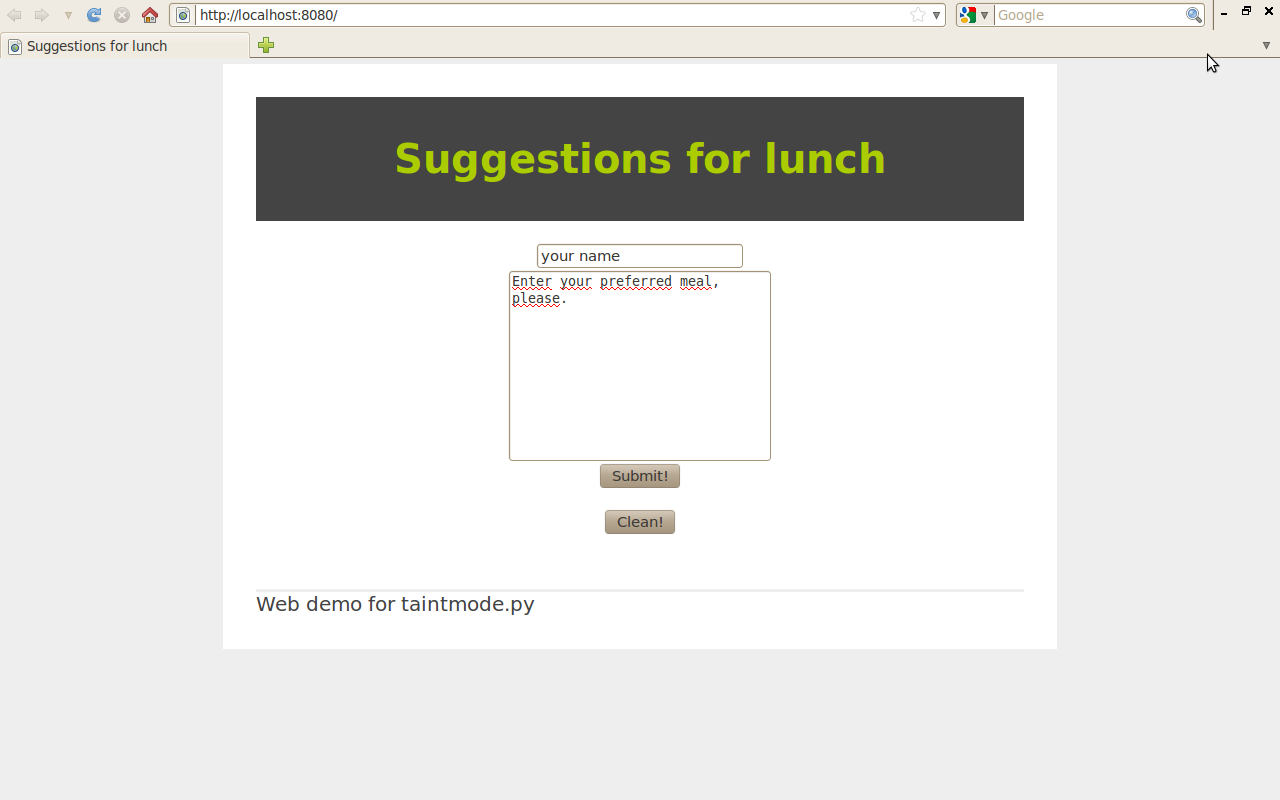
\includegraphics[width=100mm]{lunch1.png}

\suggestions is a web application supposed
to be used in an office to decide what to eat at lunch.
In the morning the employees submit theier suggestion and each day
the designed buyer check the suggestions before go to buy the food.

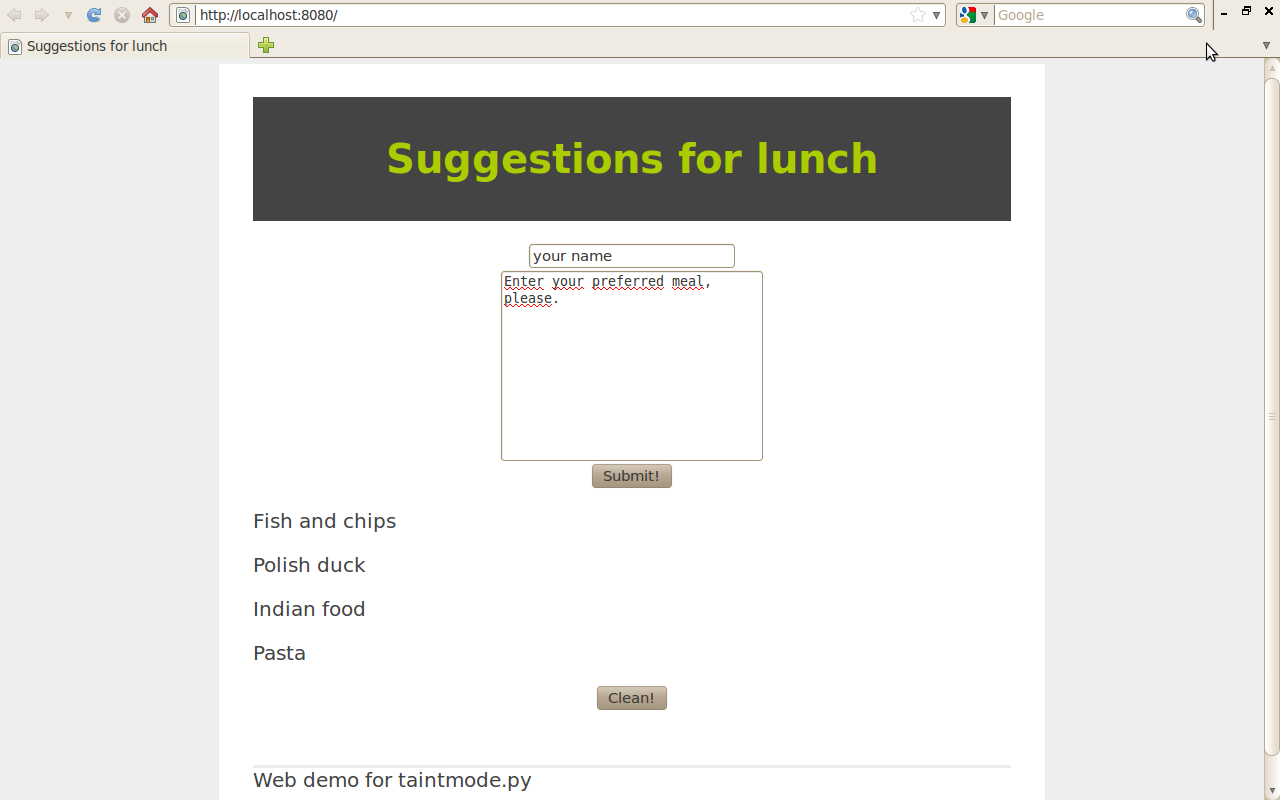
\includegraphics[width=100mm]{lunch2.png}

It seems to work prety well, but the application have a problem. It uses
as datastore a text file and use operating system facilities in order to
store de information in the file.

%\begin{wrapfigure}{c}{6.5cm}
\begin{figure}[h]
%\vspace{-25pt}
{\small{
\lstinputlisting[language=Python,numbers=left]
{lunchproblem.py}
\caption{\label{fig:example}A problem in the web application}
}}
%\vspace{-15pt}
\end{figure}
%\end{wrapfigure}


We can see that data received from the untrusted source
\texttt{web.input} is used
with no validation to build a command tha later is used
in the sensitive sink \texttt{os.system}. 
\texttt{os.system} is a Python object that let the 
programmer execute raw commands against the operating system.

\subsection*{Attacks} % va la subseccion?
\label{Sec:Attacks}
An attacker can abuse this application in order to perform different attacks.
Instead of supply his desire meal, he can submit \texttt{; ls} to make the 
executed command list the files in the application root directory and save that
list in the suggestions file:

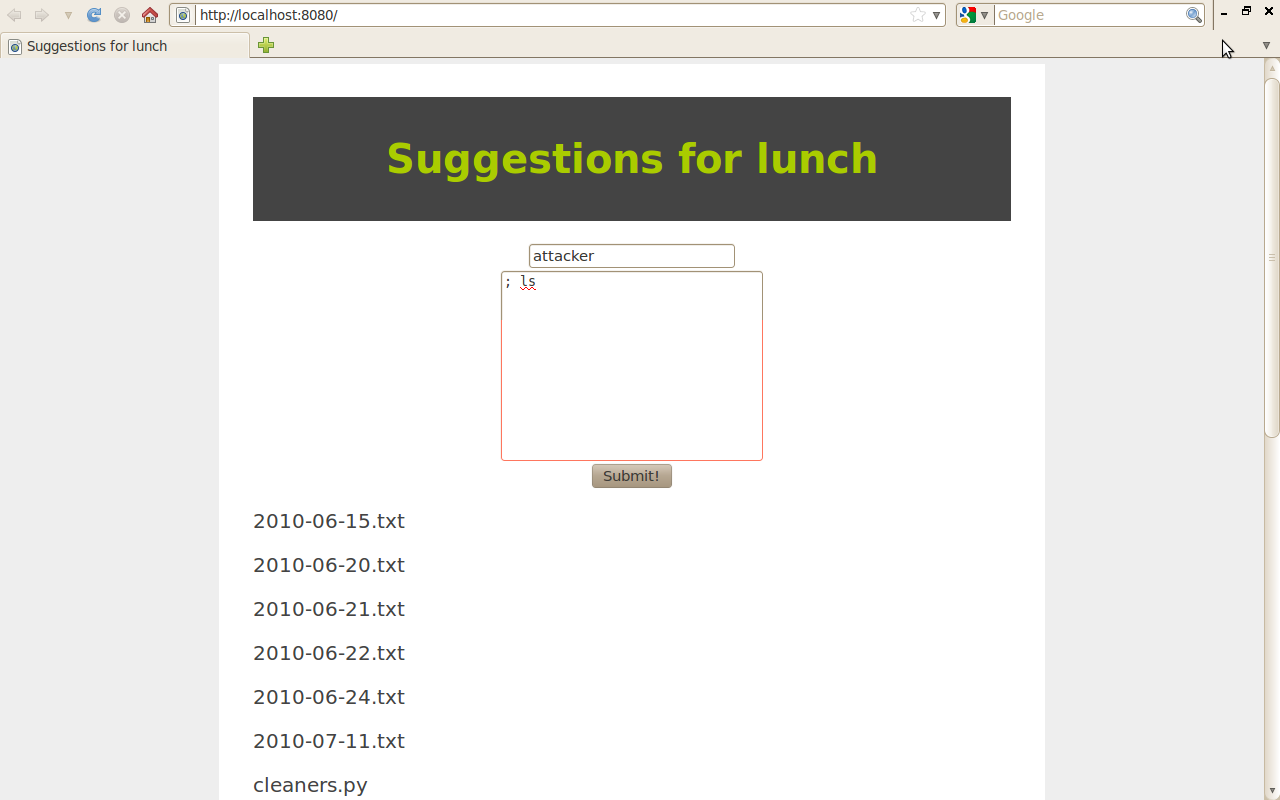
\includegraphics[width=100mm]{lunch3.png}

If he find something instresting, for example a file called 
\texttt{passwords.txt},
he can submit \texttt{; cat passwords.txt}
and read the content of that file:

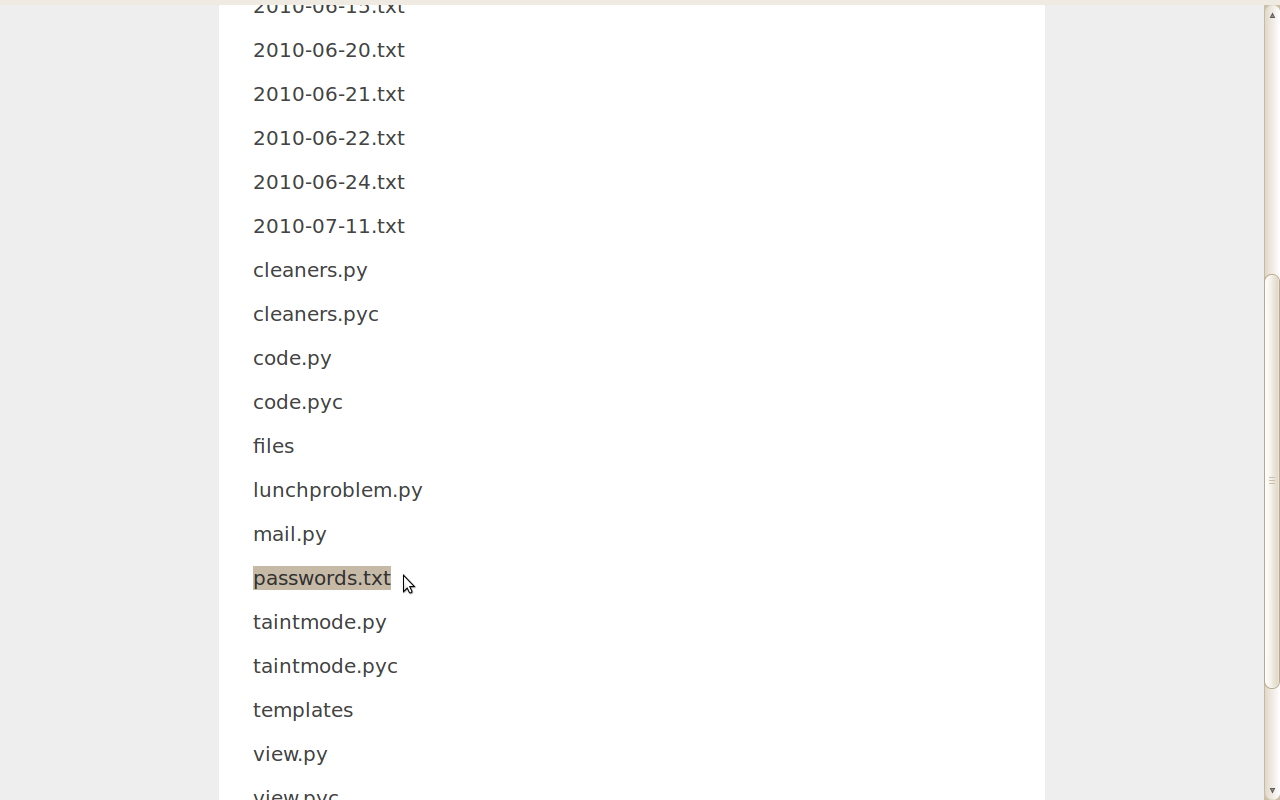
\includegraphics[width=100mm]{lunch4.png}

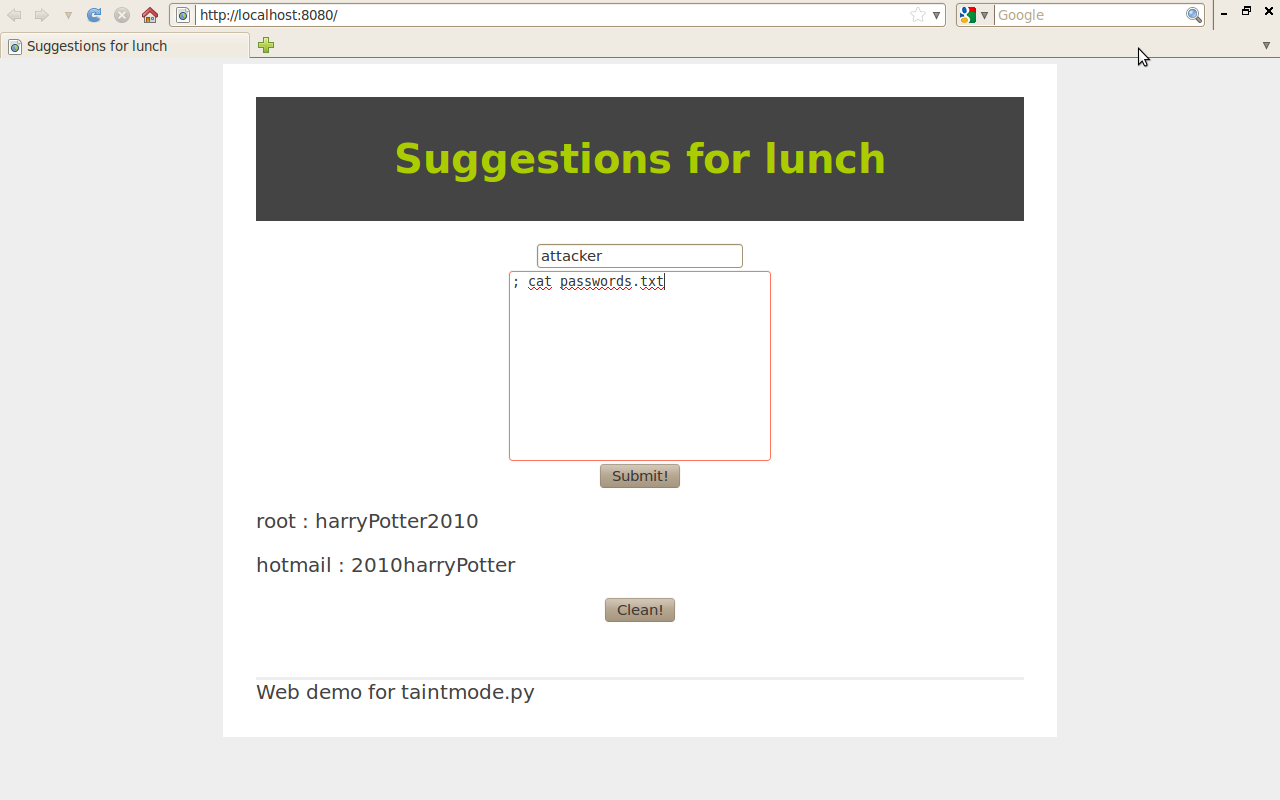
\includegraphics[width=100mm]{lunch5.png}

Even more, he can read the content of system sensitive files and,
for example, submitting \texttt{; cat /etc/passwd} get the list
of the system users:

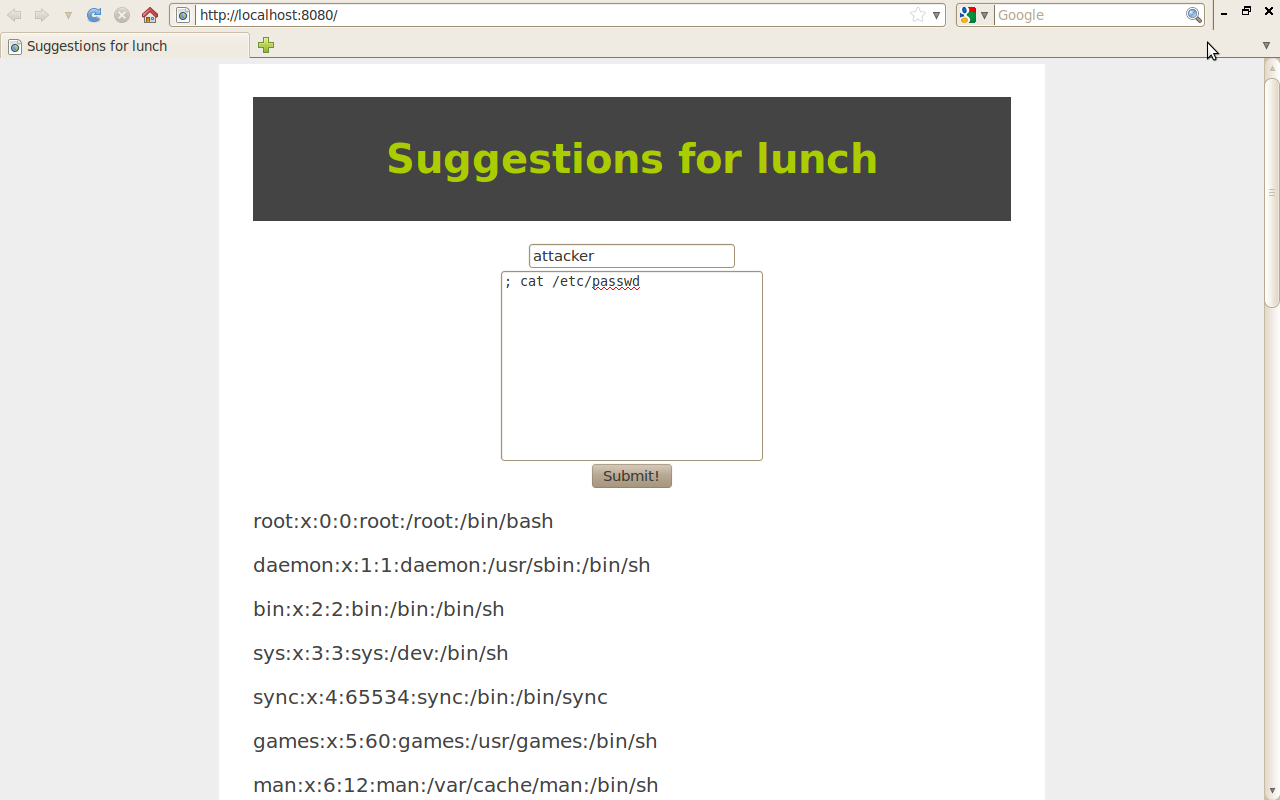
\includegraphics[width=100mm]{lunch6.png}


These attacks demonstrate how, 
what was intended to be a simple web application,  
can become a web-based file browser or a terminal. To avoid 
these vulnerabilities, applications need to rigorously check 
for malicious data provided by users or any other 
untrustworthy source. 

Taint analysis helps to detect when 
data is not sanitize before it is used on security critical 
operations. In Chapter \ref{Chap:Library}, we show how to harden 
\suggestions in order to reject the vulnerabilities 
shown in Section Attacks.

\section{Python programming language}

As its web site explains\cite{Python},
%Python is a programming language that lets programmers
%work more quickly and integrate their systems more effectively.
%Once Python is lerned gains in productivity
%and lower maintenance costs are inmidiatly seen.
Python is an interpreted, interactive, object-oriented programming language.
It incorporates modules, exceptions, dynamic typing, 
very high level dynamic data types, and classes. 
Python combines remarkable power with very clear syntax. 
It has interfaces to many system calls and libraries, as well 
as to various window systems, and is extensible in C or C++. 
It is also usable as an extension language for applications that 
need a programmable interface. Finally, Python is portable: it 
runs on many Unix variants, on the Mac, and on PCs under 
MS-DOS, Windows, Windows NT, and OS/2.

We said that the common way of implement taint mode in a programming
language is modifying the interpreter. Rather than doing this,
we present how to provide
a taint mode for Python via a library written entirely in Python. 

Python is spreading fast inside
web development \cite{WikiPython}. 
For instance, 
the popular Wiki engine 
MoinMoin (e.g. used by Ubuntu forums)
and Youtube are mostly written in Python.  Among companies, 
we can mention Google, which uses 
the language for some of its search-engine internals at
Google Groups, Gmail, and Google Maps.
There are also many numbers of web development frameworks written
in Python; Django\cite{Django}, de most popular one is widely used
in the industry and was addopted as one of the first supported
tools in Google App Engine cloud computing platform.

Besides its successful use, Python presents 
some programming languages abstractions that makes possible 
to provide a taint mode via a library. For example, 
Python decorators \cite{Lutz:1999:LP} are a non-invasive and simple 
manner to declare sources of tainted data, sensitive sinks, and 
sanitation functions. Python's 
object-oriented and dynamic typing mechanisms allows the 
execution of the taint analysis with almost no modifications in the
source code. 

The library provides a general method to enhance Python's built-in
classes with tainted values. 
%To demostrate the flexibility of our approach, 
%the library enhances the built-in classes for
%strings, integers, and floats. 
In general, taint
analysis tends to only consider strings or characters 
\cite{Perl,Nguyen05,Haldar05dynamictaint,KozlovPetukhov07,Futo07,SeoLam2010}.
% when 
%implemented as part of interpreters. 
In contrast, our library 
can be easily adapted to consider different built-in
classes
% as well as users' specific ones, 
and thus providing a taint
analysis for a wider set of data types. 
By only considering tainted strings, the library provides 
a similar analysis than in \cite{KozlovPetukhov07},
but without modifying the Python interpreter.
To the best of our knowledge, a
library for taint analysis has not been considered before. 

\section{Organization}
The rest of the thesis is organized as following. Chapter 2 describes background
knowledge, existing approaches for taint mode and the general idea of tain analysis.
Chapter 3 introduces the library, its API and shows how to use it to harden
the example application \suggestions.
Chapter 4 presents implementation details of the library with special attention
to those Python features that make it easy to build this technology in a
noninvasive way from the programmer point of view.
Chapter 5 explains limitations of the current approach and discusses alternatives.
In Chapter 6 we present conclusions and ideas for future works.
library source code as well as the example source code are provided in the Appendix.
